\documentclass[conference]{IEEEtran}
\IEEEoverridecommandlockouts

\usepackage{cite}
\usepackage{amsmath,amssymb}
\usepackage{graphicx}
\usepackage{booktabs}
\usepackage{multirow}
\usepackage{xcolor}
\usepackage{tikz}
\usetikzlibrary{arrows.meta,positioning,calc}
\usepackage[hidelinks]{hyperref}

\newcommand{\pp}{\,pp}            % percentage points
\newcommand{\A}[1]{\textsf{#1}}    % arm identifiers

\begin{document}

\title{Where Does the Gain Come From? Disentangling GAN-BERT and Affective Helper Tasks in Low-Resource Sarcasm Detection}

% Double-blind submission: no author names, affiliations or links.
\author{\IEEEauthorblockN{Anonymous Authors}
\IEEEauthorblockA{\textit{Affiliation withheld for review}}}

\maketitle

\begin{abstract}
Semi-supervised sarcasm detectors that combine GAN-BERT with sentiment and emotion helper tasks report high accuracy, but they mix three ingredients: adversarial training on unlabelled text, extra helper heads, and helper labels produced by pretrained models. We separate these ingredients in a controlled study on the News Headlines dataset. Ten training arms share one encoder, one optimiser and one step budget and are run at five label budgets (1\% to 100\%) with five seeds each; every comparison uses a paired bootstrap over test items. The GAN never improves over plain BERT, and a small sweep of its generator learning rate and training length does not change this. The gains that the combined model is credited with come from simpler sources: supervised adversarial training (FGM) adds 1.6 macro-F1 points at 1\% and 10\% labels, self-training adds 1.6 points at 1\%, and helper heads trained on the labelled rows add 1.6 points at 1\%, of which 1.2 points remain when the helper labels are shuffled. Combining the GAN with helper heads costs 2.3 points at 1\%. Helper-label quality matters only under heavy damage, and agreement with a 200-item human audit does not predict which label source helps. Finally, every model relies on outlet-specific words (masking them costs about 3 points more than masking random words), and no model transfers to iSarcasmEval, where an in-domain model reaches an AUC of 65.8.
\end{abstract}

\begin{IEEEkeywords}
sarcasm detection, semi-supervised learning, GAN-BERT, multi-task learning, adversarial training, ablation study
\end{IEEEkeywords}

% ======================================================================
\section{Introduction}

Sarcasm inverts the literal meaning of a sentence, so systems that read surface sentiment get it wrong. Labelled sarcasm data are expensive, which has made semi-supervised learning attractive. A recent line of work combines GAN-BERT~\cite{croce2020ganbert}, which learns from unlabelled text through a generator--discriminator game on BERT's sentence vector, with multi-task learning: helper heads predict the sentiment and emotion of each text, using labels produced by pretrained classifiers~\cite{irfan2025seed}. On the News Headlines dataset~\cite{misra2023sarcasm} such a model reports 93.88\% accuracy~\cite{irfan2025seed}.

That number, however, rests on three ingredients introduced together. The first is adversarial semi-supervised training. The second is the extra heads, which add training signal to the shared encoder. The third is the helper labels: because they are machine-made, they exist for every text, including those whose sarcasm label is withheld. The helper heads can therefore learn from the unlabelled pool on their own, which makes multi-task learning a semi-supervised mechanism that competes with the GAN. Which ingredient produces the gain, at which label budget, has not been measured.

We answer three questions on a single re-implementation in which only the ingredient under test changes:
\begin{itemize}
\item \textbf{RQ1:} How much of the gain over BERT comes from the GAN, from helper heads (with and without the unlabelled pool), and from both together, at label budgets from 1\% to 100\%?
\item \textbf{RQ2:} Does the quality of the machine-made helper labels matter?
\item \textbf{RQ3:} Do the models learn sarcasm or outlet style, and do they transfer to a second dataset?
\end{itemize}

Our contributions are: (i) a controlled ablation with ten arms, five budgets, five seeds and paired bootstrap tests, including two baselines the GAN must beat: supervised adversarial training (FGM)~\cite{miyato2017adversarial} and self-training~\cite{lee2013pseudo}. (ii) A label-quality study with seven helper-label variants and a 200-item human audit of the sentiment teacher. (iii) Shortcut and transfer checks: an outlet-cue masked test with a random-mask control, and evaluation on iSarcasmEval~\cite{abufarha2022semeval} against an in-domain reference. The answer is unflattering for the GAN, and it suggests where the effort in this model family should go.

% ======================================================================
\section{Related Work}

\textbf{GAN-based semi-supervised text classification.} GAN-BERT~\cite{croce2020ganbert} adds a generator that produces fake sentence vectors and a discriminator with $k{+}1$ outputs (the $k$ classes plus ``fake''), trained with feature matching~\cite{salimans2016improved}. Its own learning curves show the advantage over BERT shrinking as labelled data grow. Semi-supervised methods are known to look better than they are when baselines are weakly tuned~\cite{oliver2018realistic}. In Bengali sarcasm detection, supervised FGM fine-tuning was reported to match or beat GAN-BERT, although that comparison copied the GAN-BERT numbers from another paper~\cite{zihan2026fgm}.

\textbf{Affective helper tasks for sarcasm.} Sentiment and emotion have been used as auxiliary tasks for multimodal sarcasm~\cite{chauhan2020sentiment}, as intermediate tasks for BERT~\cite{savini2022intermediate}, and as lexicon-derived soft targets in an LSTM model~\cite{chen2022jointly}. Weak labels from pretrained models can serve as auxiliary targets in affect recognition~\cite{dai2021weakly}. These studies are fully supervised. They do not ask whether helper heads trained on unlabelled text act as a semi-supervised signal, nor how good the helper labels need to be.

\textbf{Shortcuts and transfer.} Models often exploit dataset artefacts instead of the intended task~\cite{gururangan2018annotation,geirhos2020shortcut}. In News Headlines, the label is the outlet: sarcastic items come from \textit{The Onion} and non-sarcastic ones from \textit{HuffPost}~\cite{misra2023sarcasm}. Sarcasm detectors are known to transfer poorly across datasets~\cite{jang2024generalizable}.

% ======================================================================
\section{Experimental Design}

\subsection{Data}
\textbf{News Headlines}~\cite{misra2023sarcasm}: 28,619 headlines. Following~\cite{irfan2025seed} we remove punctuation, then drop 118 duplicate copies, leaving 28,501 (47.5\% sarcastic). A fixed stratified split gives 22,800 training, 2,850 development and 2,851 test headlines. The test set was not scored until every setting had been chosen on development data. For each seed we draw nested labelled subsets $L$ of 1, 5, 10, 30 and 100\% of the training set (228 to 22,800 headlines). The rest of the training set forms the unlabelled pool $U$, whose sarcasm labels are hidden.

\textbf{iSarcasmEval}~\cite{abufarha2022semeval}: English Task~A, tweets labelled by their own authors. We use the official test set (1,400 tweets, 200 sarcastic) for transfer, and the training set (3,467 after cleaning) only to train an in-domain reference model.

\textbf{Helper labels.} As in~\cite{irfan2025seed}, sentiment comes from a Twitter-RoBERTa classifier~\cite{barbieri2020tweeteval} (3 classes) and emotion from a GoEmotions model~\cite{demszky2020goemotions}, whose 28 classes we map to five groups (joy, sadness, anger, fear, neutral/other). Both are applied once to every headline. The labels are skewed: 56\% of headlines are neutral in sentiment and 83\% fall in the neutral/other emotion group.

\subsection{Arms}
All arms share bert-base-uncased~\cite{devlin2019bert} and use the [CLS] vector $\mathbf{h}$ as the sentence representation (Fig.~\ref{fig:arch}). They differ only in the switches below. Arms A3, A4, A5, A6 and A8 also see one batch of $U$ per step.
\begin{itemize}
\item \A{A0}: TF-IDF (word 1--2 grams) with logistic regression, as a floor.
\item \A{A1}: BERT trained on $L$ only.
\item \A{A2}/\A{A3}: A1 plus linear sentiment and emotion heads on $\mathbf{h}$, with loss $\mathcal{L}_{\mathrm{sar}} + w(\mathcal{L}_{\mathrm{sent}} + \mathcal{L}_{\mathrm{emo}})$. A2 applies the helper loss to $L$ only. A3 applies it to $L{+}U$, as in~\cite{irfan2025seed}.
\item \A{A4}: GAN-BERT~\cite{croce2020ganbert}. The generator maps 100-d noise to a fake $\tilde{\mathbf{h}}$. The discriminator has $k{+}1$ outputs. The generator is trained with feature matching~\cite{salimans2016improved}.
\item \A{A5}: A4 plus the A3 helper heads, our re-implementation of the combined model. We use shared helper heads rather than the per-task generator--discriminator pairs of~\cite{irfan2025seed}, so that A5 is exactly A3 plus A4.
\item \A{A6}: one round of self-training~\cite{lee2013pseudo}. The A1 model labels $U$; items with confidence $\geq 0.9$ are kept, class-balanced, and used as a second batch.
\item \A{A7}: BERT on $L$ with FGM~\cite{goodfellow2015explaining,miyato2017adversarial}: an $\ell_2$-normalised adversarial perturbation of size $\epsilon$ on the word embeddings, adding the adversarial loss to the clean loss. This tests whether ``adversarial'' helps without a GAN.
\item \A{A8}: A3 with the helper labels shuffled across headlines (class proportions kept). \A{A9}: the same for A2.
\end{itemize}

\begin{figure}[t]
\centering
\resizebox{\columnwidth}{!}{% Shared model with the switches that define the arms (Fig. 1).
% Drawn in TikZ so fonts match the paper; colours follow the data figures.
% Needs \usetikzlibrary{arrows.meta,positioning,calc}.
\definecolor{cblue}{HTML}{2A78D6}
\definecolor{corange}{HTML}{EB6834}
\definecolor{caqua}{HTML}{1BAF7A}
\definecolor{cink}{HTML}{52514E}
\definecolor{cfill}{HTML}{F3F2EF}
\begin{tikzpicture}[
  font=\scriptsize,
  >={Stealth[length=3.5pt,width=3pt]},
  box/.style={draw=cink, fill=cfill, rounded corners=2pt, align=center, inner sep=2.2pt, minimum height=5mm, line width=0.5pt},
  head/.style={box, fill=white, minimum width=23mm},
  data/.style={box, fill=white, dashed},
  arr/.style={->, draw=cink, line width=0.5pt},
  tag/.style={font=\tiny\bfseries, inner sep=1pt},
]
% inputs, embeddings, encoder
\node[data] (L) {labelled $L$\\{\tiny headline, label $y$}};
\node[data, below=2.5mm of L.south west, anchor=north west, minimum width=0pt] (U) {unlabelled $U$\\{\tiny headline only}};
\node[box, anchor=west] (emb) at ($(L.east |- U.east)!0.5!(L.east)+(7mm,0)$) {word\\embeddings};
\node[box, right=4mm of emb, minimum height=12mm, fill=cink!12] (bert) {BERT\\encoder};
\node[circle, draw=cink, fill=white, inner sep=0.8pt, line width=0.5pt, right=3mm of bert] (h) {$\mathbf{h}$};
\draw[arr] (L.east) -- ++(2.5mm,0) |- ([yshift=1mm]emb.west);
\draw[arr] (U.east) -- ++(2.5mm,0) |- ([yshift=-1mm]emb.west);
\draw[arr] (emb) -- (bert);
\draw[arr] (bert) -- (h);
\node[tag, text=caqua, above=0.8mm of emb.north] {A7: $+\,\mathbf{r}_{\mathrm{adv}}$};

% heads on the [CLS] vector h
\path (h.east) ++(6mm, 1.45) node[head, anchor=west] (sar) {sarcasm head};
\path (h.east) ++(6mm, 0.62) node[head, anchor=west] (sen) {sentiment head (3)};
\path (h.east) ++(6mm,-0.05) node[head, anchor=west] (emo) {emotion head (5)};
\path (h.east) ++(6mm,-0.95) node[head, anchor=west] (dis) {discriminator ($k{+}1$)};
\foreach \t in {sar,sen,emo,dis} \draw[arr] (h.east) -- ++(3mm,0) |- (\t.west);

% generator under the discriminator
\node[box, fill=white, below=4.5mm of dis] (gen) {generator};
\node[left=3mm of gen] (z) {$\mathbf{z}\sim\mathcal{N}(0,I)$};
\draw[arr] (z) -- (gen);
\draw[arr] (gen) -- node[right, font=\tiny] {$\tilde{\mathbf{h}}$} (dis);

% targets
\node[font=\tiny, right=1mm of sar] {$y$ on $L$};
\node[box, fill=white, anchor=west] (teach) at ($(sen.east)!0.5!(emo.east)+(5mm,0)$) {frozen\\teachers};
\draw[arr, dashed] (teach.west) -- ++(-2.5mm,0) |- (sen.east);
\draw[arr, dashed] (teach.west) -- ++(-2.5mm,0) |- (emo.east);

% arm tags
\node[tag, text=cblue, below=0.8mm of teach] {A2, A3};
\node[tag, text=corange, right=1.5mm of gen] {A4, A5};
\end{tikzpicture}
}
\caption{Shared model. Every arm uses the same encoder and sarcasm head; the arms switch on the helper heads (A2, A3, on $L$ or $L{+}U$), the generator and $(k{+}1)$-way discriminator (A4, A5), or an adversarial embedding perturbation $\mathbf{r}_{\mathrm{adv}}$ (A7). A6 adds pseudo-labelled $U$ to the sarcasm head.}
\label{fig:arch}
\end{figure}

\subsection{Training and evaluation}
Every run uses AdamW~\cite{loshchilov2019decoupled} (weight decay 0.01), a 10\% linear warm-up then linear decay, gradient clipping at 1.0, batch size 32, maximum length 48 tokens and mixed precision. Every arm has the same number of steps, $\max(200, 10 \text{ passes over } L)$, and no early stopping, so no arm sees more labels than its budget through model selection. Three settings were chosen on development data at 10\% labels with seeds 0--2: the learning rate ($5{\times}10^{-5}$ from $\{2,3,5\}{\times}10^{-5}$, with A1), the helper weight ($w{=}0.3$ from $\{0.1, 0.3, 1\}$, with A3) and the FGM size ($\epsilon{=}0.5$ from $\{0.5,1,2\}$, with A7). The GAN arms use the published GAN-BERT design with the shared learning rate. Seeds 0--4 change the labelled subset, the initialisation and the batch order, and training is deterministic: re-running a configuration reproduces its predictions exactly. All runs used two NVIDIA T4 GPUs.

We report macro-F1 on the test set (mean $\pm$ s.d. over seeds). To compare two arms we use a paired bootstrap over test headlines~\cite{berg2012empirical}: 10,000 resamples, the same resample applied to all five seeds, the difference in seed-averaged macro-F1, a 95\% interval and a two-sided $p$. The bootstrap is the pre-set test. As a robustness check we also apply Holm's correction~\cite{holm1979simple} over the 38 research contrasts of RQ1 and the 16 contrasts of RQ2, and mark which results survive it.

% ======================================================================
\section{Results}

\begin{table*}[t]
\centering
\caption{Test macro-F1 (\%, mean $\pm$ s.d. over 5 seeds) by label budget. $^{\dagger}$: trains on the unlabelled pool $U$ (empty at 100\%). Bold: highest mean per budget (at 1\%, A2, A6 and A7 are within 0.05 points). --: not run.}
\label{tab:main}
\footnotesize
\setlength{\tabcolsep}{5pt}
\begin{tabular}{llccccc}
\toprule
 & Arm & 1\% (228) & 5\% (1,140) & 10\% (2,280) & 30\% (6,840) & 100\% (22,800) \\
\midrule
A0 & TF-IDF + logistic regression & 69.7{\scriptsize$\pm${0.7}} & 75.3{\scriptsize$\pm${0.6}} & 78.1{\scriptsize$\pm${0.6}} & 81.1{\scriptsize$\pm${0.4}} & 84.7 \\
A1 & BERT (labelled only) & 80.4{\scriptsize$\pm${1.2}} & 86.6{\scriptsize$\pm${0.5}} & 88.2{\scriptsize$\pm${0.3}} & 90.8{\scriptsize$\pm${0.2}} & \textbf{93.3}{\scriptsize$\pm${0.4}} \\
A2 & BERT + helper heads on $L$ & \textbf{82.1}{\scriptsize$\pm${0.6}} & -- & 88.4{\scriptsize$\pm${0.4}} & -- & -- \\
A3 & BERT + helper heads on $L{+}U$$^{\dagger}$ & 80.3{\scriptsize$\pm${1.8}} & \textbf{86.8}{\scriptsize$\pm${0.7}} & 88.6{\scriptsize$\pm${0.5}} & \textbf{91.1}{\scriptsize$\pm${0.4}} & -- \\
A4 & GAN-BERT$^{\dagger}$ & 80.5{\scriptsize$\pm${1.6}} & 86.5{\scriptsize$\pm${1.0}} & 88.1{\scriptsize$\pm${0.4}} & 90.3{\scriptsize$\pm${0.2}} & -- \\
A5 & GAN-BERT + helper heads$^{\dagger}$ & 78.1{\scriptsize$\pm${2.7}} & 86.6{\scriptsize$\pm${0.5}} & 88.4{\scriptsize$\pm${0.3}} & 90.8{\scriptsize$\pm${0.2}} & -- \\
A6 & Self-training$^{\dagger}$ & 82.0{\scriptsize$\pm${0.7}} & -- & 88.8{\scriptsize$\pm${0.3}} & -- & -- \\
A7 & BERT + FGM & 82.0{\scriptsize$\pm${0.6}} & -- & \textbf{89.8}{\scriptsize$\pm${0.1}} & -- & -- \\
A8 & A3, shuffled helper labels$^{\dagger}$ & 80.0{\scriptsize$\pm${1.7}} & -- & 88.1{\scriptsize$\pm${0.3}} & -- & -- \\
\bottomrule
\end{tabular}

\end{table*}

\begin{figure*}[t]
\centering
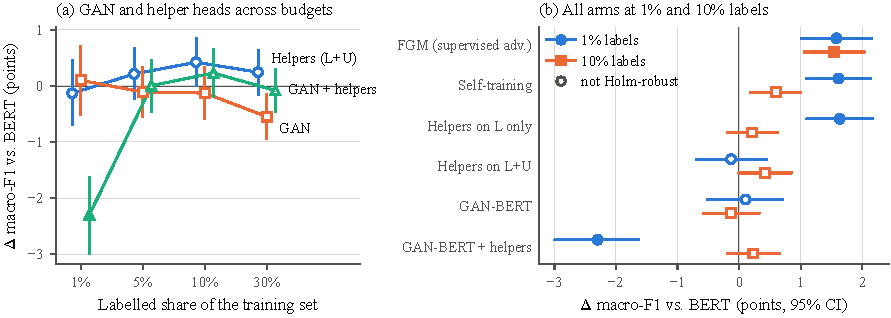
\includegraphics[width=\textwidth]{figures/fig_rq1.pdf}
\caption{RQ1: difference in test macro-F1 from BERT (A1), paired bootstrap over test items with 95\% intervals, 5 seeds. Filled markers survive Holm's correction over the 38 RQ1 contrasts; hollow markers do not. (a) The 2$\times$2 arms across budgets (horizontal offsets for legibility). (b) All arms at 1\% and 10\% labels.}
\label{fig:rq1}
\end{figure*}

\subsection{RQ1: Which ingredient gives the gain?}
Table~\ref{tab:main} gives the scores and Fig.~\ref{fig:rq1} the paired differences from BERT. BERT beats the TF-IDF floor by 8.7 to 11.3 points at every budget.

\textbf{The GAN never helps.} A4 $-$ A1 is $+0.10$, $-0.11$ and $-0.13$ points at 1, 5 and 10\% (all $p > 0.5$) and $-0.55$ at 30\% ($p = 0.007$, not robust to Holm). Because the GAN used fixed settings while FGM and the helper weight were tuned, we also ran a development-only check: generator learning rates of $10^{-5}$ and $2{\times}10^{-4}$ at 10\% labels, and three times the training steps at 1\% (with A1 given the same extra steps). We fixed the rule in advance: any setting beating the current GAN by more than one standard deviation, on every seed, would be re-run on the test set. None did. The learning-rate changes gained 0.2 development points (one standard deviation is 0.7), and longer training lowered both GAN-BERT ($-2.3$) and BERT ($-0.7$).

\textbf{Simpler methods give the gains the GAN does not.} FGM improves over BERT by $+1.58$ points at 1\% and $+1.55$ at 10\% ($p < 10^{-4}$ at both) and beats the GAN by 1.5 to 1.7 points. Self-training adds $+1.62$ at 1\% and $+0.60$ at 10\%. Both results at 1\% survive Holm.

\textbf{Helper heads help only without the unlabelled pool, and only at 1\%.} Trained on $L$ alone, the helper heads add $+1.63$ points at 1\% (robust). Adding the unlabelled pool, as the combined model does, removes this gain (A3 $-$ A2 $= -1.76$, robust). With $U$, the helper heads give a small positive effect at 5--30\% ($+0.21$ to $+0.42$) that is not significant at any budget; the largest, $+0.42$ at 10\%, has $p = 0.051$.

\textbf{The combination is harmful at 1\%.} GAN-BERT with helper heads (A5) loses 2.30 points to BERT at 1\% and has the largest seed variance in the table (s.d.\ 2.7). The 2$\times$2 interaction is $-2.27$ points (robust). From 5\% upward A5 is indistinguishable from BERT.

\subsection{RQ2: Does helper-label quality matter?}
We vary only the helper labels on the two arms where helpers mattered: A2 at 1\% and A3 at 10\%. The variants are soft teacher probabilities, 25\% and 50\% of labels flipped at random, VADER lexicon sentiment~\cite{hutto2014vader}, a second sentiment teacher (RoBERTa-large~\cite{hartmann2023more}), a single head (sentiment or emotion only) and shuffled labels (Fig.~\ref{fig:rq2}).

\begin{figure}[t]
\centering
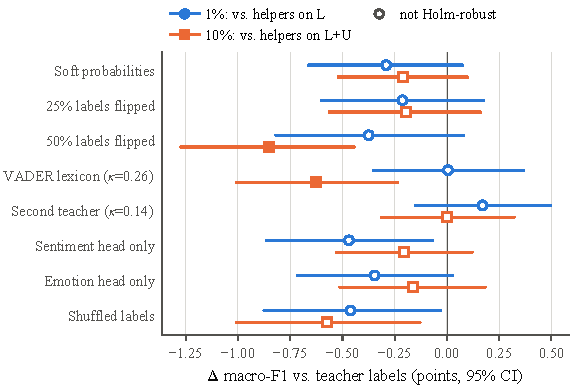
\includegraphics[width=\columnwidth]{figures/fig_rq2.pdf}
\caption{RQ2: change in test macro-F1 when only the helper labels change, against the same arm with the original teacher labels (paired bootstrap, 95\% intervals, 5 seeds). $\kappa$: agreement of each sentiment source with the human audit (teacher~1: 0.24). Filled: survives Holm over the 16 contrasts.}
\label{fig:rq2}
\end{figure}

\textbf{At 1\%, most of the helper gain is not label content.} With shuffled labels (A9), the helper heads still beat BERT by $+1.17$ points ($p < 10^{-4}$, robust), which is 72\% of the $+1.63$ obtained with real labels. Real labels add only $0.46$ points over shuffled ones ($p = 0.034$, not robust). No other variant changes A2 by more than 0.5 points.

\textbf{At 10\%, only heavy damage hurts.} Flipping half of the labels costs $0.85$ points and VADER labels cost $0.63$ (both robust). Soft labels, 25\% flips, the second teacher and either single head change nothing measurable ($|\Delta| \leq 0.21$).

\textbf{Human agreement does not predict usefulness.} We audited the sentiment sources against 200 training headlines labelled blind for surface sentiment by one annotator (Table~\ref{tab:gold}). Every source agrees only fairly with the human ($\kappa$ 0.14--0.26~\cite{cohen1960coefficient}), and the annotator marked 48\% of items as uncertain. The ordering does not carry over to training: the second teacher, with the lowest $\kappa$, costs nothing, while VADER, with the highest, is the only source that hurts. VADER's labels are also far more balanced across classes than the teacher's (negative/neutral/positive 33/34/32\% against 33/56/11\% on the training set), which may matter more than its accuracy.

\textbf{Helper labels carry little sarcasm signal.} On the training set, sentiment and emotion labels share almost no information with the sarcasm label (normalised mutual information 0.004 and 0.002), and a logistic probe on the eight teacher probabilities predicts sarcasm at an AUC of only 0.546. On the audit items, neither the human's sentiment labels (AUC 0.458) nor the teacher's (0.496) predict sarcasm. The helper heads therefore do not pass a hidden shortcut to the sarcasm head. Together with the shuffled-label result, this suggests they act mainly as a regulariser on the shared encoder when labels are scarce.

\begin{table}[t]
\centering
\caption{Sentiment sources against the human audit (200 training headlines, 3 classes). Sure: the 104 items the annotator did not mark as uncertain.}
\label{tab:gold}
\footnotesize
\setlength{\tabcolsep}{4pt}
\begin{tabular}{lcccc}
\toprule
Source & Acc. & Macro-F1 & $\kappa$ & $\kappa$ (sure) \\
\midrule
Teacher 1 (used in training) & 53.0 & 49.1 & 0.24 & 0.25 \\
VADER lexicon & 50.5 & 50.3 & 0.26 & 0.37 \\
Teacher 2 (RoBERTa-large) & 48.0 & 42.7 & 0.14 & 0.13 \\
\bottomrule
\end{tabular}

\end{table}

\begin{figure*}[t]
\centering
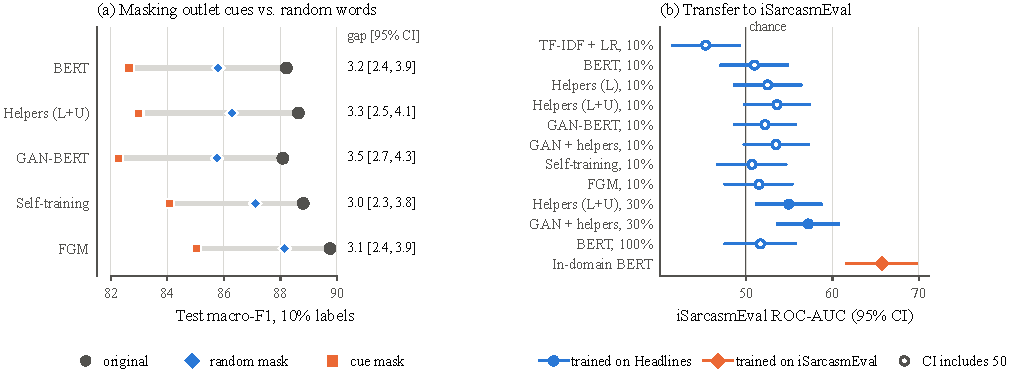
\includegraphics[width=\textwidth]{figures/fig_rq3.pdf}
\caption{RQ3. (a) Test macro-F1 at 10\% labels on the original test set, after masking the same number of random words, and after masking the 200 most outlet-indicative words; the gap is random-mask minus cue-mask F1 (paired bootstrap). (b) ROC-AUC on the iSarcasmEval test set with 95\% bootstrap intervals; filled: interval excludes 50. In-domain BERT is trained on iSarcasmEval.}
\label{fig:rq3}
\end{figure*}

\subsection{RQ3: Sarcasm or outlet style?}
\textbf{Outlet cues.} We trained a unigram logistic regression on the full training set and took the 100 words most indicative of each outlet. The list was fixed before any masked score was seen; its top words are style markers such as \textit{area}, \textit{local}, \textit{report} (\textit{The Onion}) and \textit{donald}, \textit{why} (\textit{HuffPost}). We replaced these words with [MASK] in the test set, which touches 62\% of test headlines (1.6 words each on average). As a control, we masked the same number of randomly chosen words in each headline. Every Headlines-trained model loses 4.7 to 5.8 points under cue masking but only 1.6 to 2.8 under random masking. The difference of about 3 points ($p < 10^{-4}$) is the same for all methods (Fig.~\ref{fig:rq3}a) and for all 15 helper-label variants. FGM and self-training lose less overall, but they also lose less under random masking, so they are more robust to missing words, not less dependent on outlet words. A model trained on iSarcasmEval shows no gap on the masked Headlines test (0.5 points, $p = 0.22$), so the gap reflects what the Headlines models learned rather than damage done by the masking.

\textbf{Transfer.} On iSarcasmEval, every Headlines-trained BERT model scores near chance (ROC-AUC 47 to 57; Fig.~\ref{fig:rq3}b), and the TF-IDF floor scores below chance. A BERT model trained on the iSarcasmEval training set reaches 65.8 [61.6, 69.8], so the test set is learnable. Only four of the 41 Headlines-trained BERT configurations have an interval above 50. All four train helper heads on $L{+}U$ (e.g., A5 at 30\%: 57.2 [53.6, 60.7]), but they remain far below the in-domain model, and no correction for multiple comparisons was applied.

% ======================================================================
\section{Discussion}

\textbf{Where does the gain come from?} Not from the GAN. In our setting the generator--discriminator game adds nothing at any budget. When it is combined with helper heads at 1\%, it makes training unstable and loses 2.3 points. The useful parts of the combined model are better obtained separately. If labels are very scarce, helper heads on the labelled rows, self-training or FGM each give about 1.6 points. FGM is the only method that also helps at 10\%, and it needs no unlabelled data. Most of the helper-head gain survives label shuffling, so it should not be read as ``sentiment and emotion knowledge helps sarcasm''. It is closer to a regularisation effect of predicting any consistent auxiliary target. This also explains why the quality of the helper labels hardly matters.

\textbf{What the scores measure.} On News Headlines all models rely on outlet vocabulary, to the same degree, and none transfers to author-labelled sarcasm on Twitter. High in-domain accuracy on this dataset is therefore weak evidence of sarcasm understanding. Because the shortcut affects every arm equally, the comparisons between arms remain valid. Absolute scores and claims of sarcasm detection should be reported with this caveat.

\textbf{Limitations.} (i) The GAN arms used published settings. FGM and the helper weight were each chosen from three values. Our GAN check covers two generator learning rates and a longer schedule, not a full search. (ii) Our combined model is a re-implementation. The original code and several settings of~\cite{irfan2025seed} were unavailable, and we used shared helper heads, so our absolute numbers are not comparable with the reported 93.88\% accuracy. (iii) The human audit has a single annotator who knew the hypotheses, although labelling was blind to the sarcasm and teacher labels. Agreement in the first 50 items was lower than later (a warm-up effect), so the audit gives a rough quality level rather than a precise one. (iv) We study one encoder, one main dataset and one transfer set. Prediction files store probabilities to six decimals, which introduces ties in the transfer AUCs (up to 1.3 points per seed for the most confident models). This does not change any conclusion.

% ======================================================================
\section{Conclusion}

Combining GAN-BERT with affective helper tasks looks like a strong semi-supervised sarcasm detector. Taken apart under one protocol, its gain does not come from the GAN. Helper heads help when labels are very scarce, mostly as a regulariser rather than through what their labels say. Supervised adversarial training and self-training are simpler, at least as effective, and more stable. On News Headlines, all methods learn outlet style to the same degree and none transfers to iSarcasmEval. Future work on this model family should use datasets whose labels are not tied to the source, and should report ablations of each ingredient alongside the full model.

\bibliographystyle{IEEEtran}
\bibliography{refs}

\end{document}
